\section{Đề ôn thi giữa kỳ 2 toán 10}
\subsection{Phần trắc nghiệm}
Câu trắc nghiệm nhiều phương án lựa chọn. Học sinh trả lời từ câu 1 đến câu 12. Mỗi câu hỏi học sinh \textit{chỉ chọn một} phương án.

\Opensolutionfile{ans}[Ans/Dapan]

\hienthiloigiaiex
%%%=============EX_1=============%%%
\begin{ex}%[0D3N2-2]%[Dự án đề kiểm tra Toán khối 10 GHKII NH23-24-Đợt 2-Viết Tường]%[Đề số 5-KNTT]
	\immini{
		Cho hàm số $y=f(x)$ có đồ thị như hình vẽ bên. Khẳng định nào sau đây \textbf{sai}?
		\choice 
		{Hàm số đồng biến trên $(-1;1)$} 
		{Hàm số nghịch biến trên $(-1;1)$}
		{Hàm số đồng biến trên $(-2;0)$} 
		{\True Hàm số đồng biến trên $(0;1)$}
	}{
		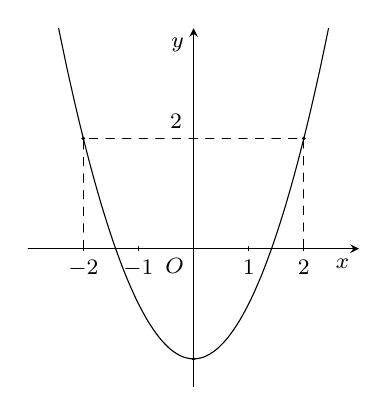
\begin{tikzpicture}[font=\footnotesize ,line cap=round,line join=round,scale=.7,>=stealth]
			\draw[->] (-3,0)--(3,0) node[below left] {$x$};
			\draw[->] (0,-2.5)--(0,4) node[below left] {$y$};
			\draw (0,0) node [below left] {$O$};
			\foreach \x in {-2,-1,1,2}
			\draw[thin] (\x,1pt)--(\x,-1pt) node[below] {$\x$};
			\foreach \y in {2}
			\draw[thin] (1pt,\y)--(-1pt,\y) node[above left] {$\y$};
			\begin{scope}
				\clip (-3,-2.5) rectangle (3,4);
				\draw[domain=-2.5:2.5,smooth,variable=\x] plot (\x,{(\x)^2-2});
			\end{scope}
			\draw[dashed,thin](-2,0)--(-2,2)--(2,2)--(2,0);
			\coordinate (A) at (-2,2);
			\coordinate (B) at (0,-2);
			\coordinate (C) at (2,2);
			\foreach \x in {A,B,C}
			\fill[black](\x) circle (1pt);
		\end{tikzpicture}
	}
	\loigiai
	{
		Dựa vào đồ thị hàm số, ta có hàm số đồng biến trên $(0;+\infty )$.\\
		Mà $(0;1)\subset (0;+\infty )$. Nên hàm số đã cho đồng biến trên $(0;1)$.
	}
\end{ex}

\begin{ex}%[0D3N1-2]%[Dự án đề kiểm tra Toán khối 10 GHKII NH23-24-Đợt 2-Viết Tường]%[Đề số 5-KNTT]
	Tập xác định của hàm số $y=\dfrac{1}{x^2-6x+9}$ là
	\choice 
	{$(-\infty ;3)$} 
	{$(3;+\infty )$}
	{\True $\mathbb{R}\setminus \{3\}$} 
	{$\mathbb{R}$}
	\loigiai
	{
		Hàm số xác định $\Leftrightarrow x^2-6x+9\ne 0\Leftrightarrow (x-3)^2\ne 0\Leftrightarrow x\ne 3$.\\
		Vậy tập xác định của hàm số là $\mathscr D=\mathbb{R}\setminus\{3\}$.
	}
\end{ex}

\begin{ex}%[0D3H1-1]%[Dự án đề kiểm tra Toán khối 10 GHKII NH23-24-Đợt 2-Viết Tường]%[Đề số 5-KNTT]
	Hình vẽ nào sau đây \textbf{không} biểu diễn đồ thị của một hàm số?
	\choice 
	{\begin{tikzpicture}[font=\footnotesize ,line cap=round,line join=round,scale=.7,>=stealth]
			\draw[->] (-3,0)--(3,0) node[below left] {$x$};
			\draw[->] (0,-1)--(0,3) node[below left] {$y$};
			\draw (0,0) node [below left] {$O$};
			\foreach \x in {-2,2}
			\draw[thin] (\x,1pt)--(\x,-1pt) node[below] {$\x$};
			\foreach \y in {1}
			\draw[thin] (1pt,\y)--(-1pt,\y) node[above left] {$\y$};
			\begin{scope}
				\clip (-3,-1) rectangle (3,3);
				\draw[domain=0:2.5,smooth,variable=\x] plot (\x,{0.5*\x});
				\draw[domain=-2.5:0,smooth,variable=\x] plot (\x,{-0.5*\x});
			\end{scope}
			\draw[dashed,thin](-2,0)--(-2,1)--(2,1)--(2,0);
	\end{tikzpicture} }
	{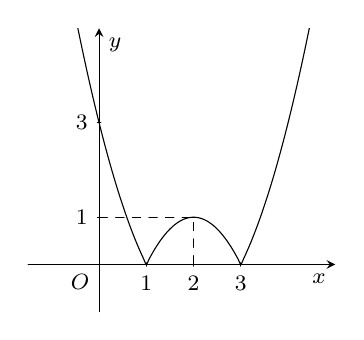
\begin{tikzpicture}[font=\footnotesize ,line cap=round,line join=round,scale=.6,>=stealth]
			\draw[->] (-1.5,0)--(5,0) node[below left] {$x$};
			\draw[->] (0,-1)--(0,5) node[below right] {$y$};
			\draw (0,0) node [below left] {$O$};
			\foreach \x in {1,2,3}
			\draw[thin] (\x,1pt)--(\x,-1pt) node[below] {$\x$};
			\foreach \y in {1,3}
			\draw[thin] (1pt,\y)--(-1pt,\y) node[left] {$\y$};
			\begin{scope}
				\clip(-1,-1) rectangle (5,5);
				\draw[smooth,samples=100,domain=-1:4.5] plot(\x,{abs((\x)^(2)-4*(\x)+3)});
			\end{scope}
			\draw[dashed,thin](0,1)--(2,1)--(2,0);
	\end{tikzpicture}}
	{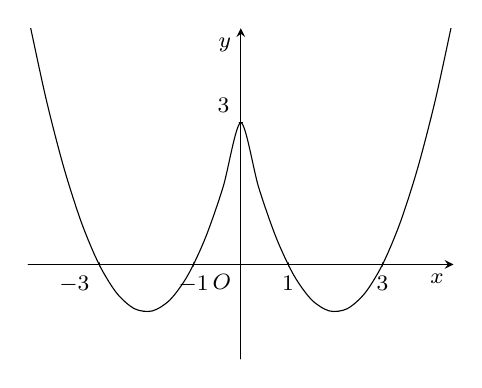
\begin{tikzpicture}[font=\footnotesize ,line cap=round,line join=round,scale=.6,>=stealth]
			\draw[->] (-4.5,0)--(4.5,0) node[below left] {$x$};
			\draw[->] (0,-2)--(0,5) node[below left] {$y$};
			\draw (0,0) node [below left] {$O$};
			\foreach \x in {-1,1,3}
			\draw[thin] (\x,1pt)--(\x,-1pt) node[below] {$\x$};
			\draw[thin] (-3,1pt)--(-3,-1pt) node[below left] {$-3$};
			\foreach \y in {3}
			\draw[thin] (1pt,\y)--(-1pt,\y) node[above left] {$\y$};
			\begin{scope}
				\clip (-4.5,-2) rectangle (4.5,5);
				\draw[domain=-4.5:4.5,smooth,variable=\x] plot (\x,{(\x)^2-4*(abs(\x))+3)});
			\end{scope}
	\end{tikzpicture}} 
	{\True \begin{tikzpicture}[font=\footnotesize ,line cap=round,line join=round,scale=1,>=stealth]
			\draw[->] (-2,0)--(2,0) node[below left] {$x$};
			\draw[->] (0,-2)--(0,2) node[below left] {$y$};
			\draw (0,0) node [below left] {$O$};
			\draw[thin] (-1,1pt)--(-1,-1pt) node[below left] {$-1$};
			\draw[thin] (1,1pt)--(1,-1pt) node[below right] {$1$};
			\foreach \y in {1}
			\draw[thin] (1pt,\y)--(-1pt,\y) node[above left] {$\y$};
			\draw[thin] (1pt,-1)--(-1pt,-1) node[below left] {$-1$};
			\draw (0,0) circle (1);
	\end{tikzpicture}}
	\loigiai
	{
		\immini{
			Xét đồ thị như hình vẽ bên.\\
			Theo định nghĩa hàm số, ứng với một giá trị của $x$ ta tìm được chỉ một giá trị của $y$.\\
			Trong đồ thị bên, với $x=0$ ta được $y=1$ và $y=-1$. Do đó đồ thị trong hình vẽ bên không phải là đồ thị của hàm số.
		}{
			\begin{tikzpicture}[font=\footnotesize ,line cap=round,line join=round,scale=1,>=stealth]
				\draw[->] (-2,0)--(2,0) node[below left] {$x$};
				\draw[->] (0,-2)--(0,2) node[below left] {$y$};
				\draw (0,0) node [below left] {$O$};
				\draw[thin] (-1,1pt)--(-1,-1pt) node[below left] {$-1$};
				\draw[thin] (1,1pt)--(1,-1pt) node[below right] {$1$};
				\foreach \y in {1}
				\draw[thin] (1pt,\y)--(-1pt,\y) node[above left] {$\y$};
				\draw[thin] (1pt,-1)--(-1pt,-1) node[below left] {$-1$};
				\draw (0,0) circle (1);
			\end{tikzpicture}
		}
	}
\end{ex}

\begin{ex}%[0D3H2-2]%[Dự án đề kiểm tra Toán khối 10 GHKII NH23-24-Đợt 2-Viết Tường]%[Đề số 5-KNTT]
	Cho $(P)\colon y=x^2-4x+11$. Khẳng định nào sau đây \textbf{sai}?
	\choice 
	{$(P)$ không cắt trục hoành} 
	{Hàm số đồng biến trên khoảng $(2;+\infty )$ và nghịch biến trên khoảng $(-\infty ;2)$}
	{Trục đối xứng của $(P)$ nằm bên phải trục tung} 
	{\True Giá trị lớn nhất của hàm số là $2$}
	\loigiai
	{
		Ta có $y=x^2-4x+11=(x-2)^2+7\ge 7$.\\
		Do đó giá trị lớn nhất của hàm số là $7$.\\
		Vậy khẳng định ``Giá trị lớn nhất của hàm số là $2$'' là \textbf{sai}.
	}
\end{ex}

\begin{ex}%[0D7H1-2]%[Dự án đề kiểm tra Toán khối 10 GHKII NH23-24-Đợt 2-Viết Tường]%[Đề số 5-KNTT]
	Cho tam thức bậc hai $f(x)=-2x^2+8x-8$. Trong các mệnh đề sau, mệnh đề nào đúng?
	\choice 
	{$f(x)<0$ với mọi $x\in\mathbb{R}$} 
	{\True $f(x)\le 0$ với mọi $x\in\mathbb{R}$}
	{$f(x)\ge 0$ với mọi $x\in\mathbb{R}$} 
	{$f(x)>0$ với mọi $x\in\mathbb{R}$}
	\loigiai
	{
		Ta có $\Delta '=4^2-(-2)\cdot (-8)=0$.\\
		Vì $\Delta =0$ và hệ số $a=-2<0$. Nên $f(x)\ge 0$ với mọi $x\in\mathbb{R}$.
	}
\end{ex}

\begin{ex}%[0D3H1-2]%[Dự án đề kiểm tra Toán khối 10 GHKII NH23-24-Đợt 2-Viết Tường]%[Đề số 5-KNTT]
	Điều kiện xác định của phương trình $\sqrt{x-1}+\sqrt{x-2}=\sqrt{x-3}$ là
	\choice 
	{$x\in (3;+\infty )$} 
	{$x\in [2;+\infty )$}
	{$x\in [1;+\infty )$} 
	{\True $x\in [3;+\infty )$}
	\loigiai
	{
		Phương trình đã cho xác định $\Leftrightarrow\heva{& x-1\ge 0\\&x-2\ge 0\\&x-3\ge 0 }\Leftrightarrow \heva{& x\ge 1\\&x\ge 2\\&x\ge 3 }\Leftrightarrow x\ge 3$.\\
		Vậy điều kiện xác định của phương trình là $x\in [3;+\infty )$.
	}
\end{ex}

\begin{ex}%[0H9N3-1]%[Dự án đề kiểm tra Toán khối 10 GHKII NH23-24-Đợt 2-Viết Tường]%[Đề số 5-KNTT]
	Trong mặt phẳng tọa độ $Oxy$, cho đường thẳng $\Delta\colon -x+2y-2=0$. Trong các véc-tơ sau, véc-tơ nào là véc-tơ chỉ phương của $\Delta$?
	\choice 
	{$\overrightarrow{u}=(-1;2)$} 
	{\True $\overrightarrow{v}=(-2;-1)$}
	{$\overrightarrow{m}=(-2;1)$} 
	{$\overrightarrow{n}=(1;2)$}
	\loigiai
	{
		$\Delta$ có véc-tơ pháp tuyến là $\overrightarrow{u}=(-1;2)\Rightarrow \overrightarrow{v}=(-2;-1)$ là véc-tơ chỉ phương của $\Delta$.
	}
\end{ex}

\begin{ex}%[0H9H3-2]%[Dự án đề kiểm tra Toán khối 10 GHKII NH23-24-Đợt 2-Viết Tường]%[Đề số 5-KNTT]
	Phương trình tham số của đường thẳng $d\colon \dfrac{x}{4}-\dfrac{y}{3}=1$ là
	\choice 
	{$\heva{& x=4+3t\\&y=4t }$} 
	{$\heva{& x=4-4t\\&y=3t }$}
	{\True $\heva{& x=4+4t\\&y=3t }$} 
	{$\heva{& x=4-3t\\&y=4t }$}
	\loigiai
	{
		$d\colon \dfrac{x}{4}-\dfrac{y}{3}=1\Rightarrow d\colon 3x-4y-12=0$.\\
		$d$ có véc-tơ pháp tuyến $\overrightarrow{u}=(3;-4)\Rightarrow d$ có véc-tơ chỉ phương $\overrightarrow{v}=(4;3)$.\\
		Mặt khác ta có $3\cdot 4-4\cdot 0-12=0\Rightarrow A(4;0)\in d$.\\
		Vậy $d\colon\heva{& x=4+4t\\&y=3t. }$
	}
\end{ex}

\begin{ex}%[0H9H3-4]%[Dự án đề kiểm tra Toán khối 10 GHKII NH23-24-Đợt 2-Viết Tường]%[Đề số 5-KNTT]
	Với giá trị nào của tham số $m$ thì hai đường thẳng $\Delta_1\colon x-2y+1=0$ và $\Delta_2\colon\heva{& x=-1+mt\\&y=2-(m+1)t }$ vuông góc với nhau?
	\choice 
	{$m=-2$} 
	{$m=2$}
	{$m=-1$} 
	{\True $m=1$}
	\loigiai
	{
		$\Delta_1$ có véc-tơ chỉ phương $\overrightarrow{u}_1=(2;1)$, $\Delta_2$ có véc-tơ chỉ phương $\overrightarrow{u}_2=(m;-m-1)$.\\
		$\Delta_1\perp\Delta_2\Leftrightarrow \overrightarrow{u}_1\cdot\overrightarrow{u}_2=0\Leftrightarrow 2m-(m+1)=0\Leftrightarrow m=1$.
	}
\end{ex}

\begin{ex}%[0H9H3-4]%[Dự án đề kiểm tra Toán khối 10 GHKII NH23-24-Đợt 2-Viết Tường]%[Đề số 5-KNTT]
	Cô-sin góc giữa hai đường thẳng $\Delta_1\colon -x+3y-1=0$ và $\Delta_2\colon\heva{& x=2+t\\&y=1-2t }$ bằng
	\choice 
	{$\dfrac{\sqrt{5}}{10}$} 
	{$\dfrac{\sqrt{10}}{10}$}
	{\True $\dfrac{\sqrt{2}}{10}$} 
	{$\dfrac{\sqrt{5}}{2}$}
	\loigiai
	{
		$\Delta_1$, $\Delta_2$ có véc-tơ chỉ phương lần lượt là $\overrightarrow{u}_1=(3;1)$ và $\overrightarrow{u}_2=(1;-2)$.\\
		$\cos\left (\Delta_1,\Delta_2 \right )=\left |\cos\left (\overrightarrow{u}_1,\overrightarrow{u}_2 \right ) \right |=\dfrac{\left |\overrightarrow{u}_1\cdot\overrightarrow{u}_2 \right |}{\left |\overrightarrow{u}_1 \right |\cdot\left |\overrightarrow{u}_2 \right |}=\dfrac{\left |3\cdot 1+1\cdot (-2) \right |}{\sqrt{3^2+1^2}\cdot\sqrt{1^2+(-2)^2}}=\dfrac{\sqrt{2}}{10}$.
	}
\end{ex}

\begin{ex}%[0H9N4-2]%[Dự án đề kiểm tra Toán khối 10 GHKII NH23-24-Đợt 2-Viết Tường]%[Đề số 5-KNTT]
	Phương trình đường tròn tâm $I(3;-2)$ và đi qua điểm $M(-1;1)$ là
	\choice 
	{$(x+3)^2+(y-2)^2=5$} 
	{\True $(x-3)^2+(y+2)^2=25$}
	{$(x-3)^2+(y+2)^2=5$} 
	{$(x-3)^2+(y-2)^2=25$}
	\loigiai
	{
		Đường tròn $(C)$ tâm $I(3;-2)$ và đi qua điểm $M(-1;1)$ có bán kính $R=IM=5\Rightarrow (C)\colon (x-3)^2+(y+2)^2=25$.
	}
\end{ex}

\begin{ex}%[0H9H4-2]%[Dự án đề kiểm tra Toán khối 10 GHKII NH23-24-Đợt 2-Viết Tường]%[Đề số 5-KNTT]
	Phương trình đường tròn $(C)$ có đường kính $AB$ với $A(-1;2)$ và $B(3;2)$ là
	\choice 
	{$(x+1)^2+(y+2)^2=4$} 
	{$(x+1)^2+(y-2)^2=16$}
	{\True $(x-1)^2+(y-2)^2=4$} 
	{$(x-3)^2+(y-2)^2=16$}
	\loigiai
	{
		Gọi $I$ là trung điểm $AB\Rightarrow I\left (\dfrac{-1+3}{2};\dfrac{2+2}{2} \right )$ hay $I(1;2)$.\\
		$(C)$ có tâm $I(1;2)$ bán kính $R=\dfrac{AB}{2}=2\Rightarrow (C)\colon (x-1)^2+(y-2)^2=4$.
	}
\end{ex}

\Closesolutionfile{ans}
\bangdapan{Dapan}

\subsection{Câu trắc nghiệm đúng sai}
Học sinh trả lời từ câu 1 đến câu 4.
Trong mỗi ý \circlenum{A}, \circlenum{B}, \circlenum{C} và \circlenum{D} ở mỗi câu, học sinh chọn đúng hoặc sai.
\setcounter{ex}{0}
\LGexTF
\Opensolutionfile{ansbook}[ansbook/DapanDS]
\Opensolutionfile{ans}[Ans/DapanT]
	%%%============EX_1==============%%%
\begin{ex}%[0D3H2-3]%[Dự án đề kiểm tra Toán khối 10 GHKII NH23-24-Đợt 2-Nguyễn Hoàng Việt]%[Đề số 5 - KNTT]
	Cho hàm số $y=x^2-6 x+5$. Khi đó:
	\choiceTF
	{Đồ thị của hàm số có toạ độ đỉnh $I(3 ; 4)$}
	{\True Đồ thị của hàm số có trục đối xứng là $x=3$}
	{Giao điểm của đồ thị với trục hoành là $A(2 ; 0)$ và $B(4 ; 0)$}
	{\True Giao điểm của đồ thị với trục tung là $C(0 ; 5)$}
	\loigiai
	{
		\begin{itemize}
			\item Ta có $a=1>0$ nên parabol quay bề lõm lên trên, có tọa độ đỉnh $I(3 ;-4)$.
			\item Ta có $a=1>0$ nên parabol quay bề lõm lên trên, có trục đối xứng là $x=3$.
			\item Giao điểm của đồ thị với trục hoành là $A(1 ; 0)$ và $B(5 ; 0)$.
			\item Giao điểm của đồ thị với trục tung là $C(0 ; 5)$.
		\end{itemize}
	}
\end{ex}

%%============EX_2==============%%
\begin{ex}%[0D7H3-1]%[Dự án đề kiểm tra Toán khối 10 GHKII NH23-24-Đợt 2-Nguyễn Hoàng Việt]%[Đề số 5 - KNTT]
	Cho phương trình $(x + 1)\left(\sqrt{x+4}- \sqrt{-x^2+4 x+14}\right) = 0$ (*). Khi đó:
	
	\choiceTF
	{Điều kiện: $x \geq 4$}
	{\True Phương trình (*) có $3$ nghiệm phân biệt}
	{Các nghiệm của phương trình (*) nhỏ hơn $5$}
	{\True Tổng các nghiệm của phương trình (*) bằng $2$}
	\loigiai
	{Điều kiện: \begin{eqnarray*}
			& & \heva{&x + 4 \geq 0\\&-x^2 + 4x + 14 \geq 0}\\ 
			&\Leftrightarrow &  \heva{&x \geq -4\\&2 -3\sqrt{2} \leq x \leq 2 + 3\sqrt{2}}\\ &\Leftrightarrow &  2 -3\sqrt{2} \leq x \leq 2 + 3\sqrt{2}.\\
		\end{eqnarray*}
		Ta có: $(x+1)\left(\sqrt{x+4}-\sqrt{-x^2+4 x+14}\right)=0 \Leftrightarrow \heva{&x+1=0 \\& \sqrt{x+4} - \sqrt{-x^2+4 x+14}= 0.}$\\
		Phương trình $x+1=0$ có nghiệm là $x=-1$.\\
		Ta có $\sqrt{x+4}-\sqrt{-x^2+4 x+14}=0 \Leftrightarrow \sqrt{x+4}=\sqrt{-x^2+4 x+14}$ (1).\\
		Bình phương hai vế phương trình (1) ta có: 
		$$x+4=-x^2+4 x+14 \Leftrightarrow x^2-3 x-10=0 \Leftrightarrow \hoac{&x = 5\\&x=-2.}$$
		Vậy tập nghiệm của phương trình ban đầu là $S=\{-2 ;-1 ; 5\}$.
		\begin{itemize}
			\item Suy ra điều kiện $x \geq 4$ là sai.
			\item Phương trình (*) có $3$ nghiệm phân biệt là đúng.
			\item Các nghiệm của phương trình (*) nhỏ hơn $5$ là sai.
			\item Tổng các nghiệm của phương trình (*) bằng $2$ là đúng.
		\end{itemize}
	}
\end{ex}

%%============EX_3==============%%
\begin{ex}%[0H9V3-7]%[Dự án đề kiểm tra Toán khối 10 GHKII NH23-24-Đợt 2-Nguyễn Hoàng Việt]%[Đề số 5 - KNTT]
	Cho tam giác $ABC$ có phương trình của đường thẳng $BC$ là $7x + 5y - 8 = 0$, phương trình các đường cao kẻ từ $B$, $C$ lần lượt là $9x - 3y - 4 = 0$, $x + y - 2 = 0$. Khi đó:
	\choiceTF
	{\True Điểm $B$ có toạ độ là $\left(\dfrac{2}{3} ; \dfrac{2}{3}\right)$}
	{\True Điểm $C$ có toạ độ là $(-1 ; 3)$}
	{Phương trình đường cao kẻ từ $A$ là $5x - 7y - 6 = 0$}
	{Phương trình đường trung tuyến kẻ từ $A$ là $x - 13y + 4 = 0$}
	\loigiai
	{Toạ độ của điểm $B$ là nghiệm của hệ phương trình:\\
		$$\heva{&7x + 5y - 8 = 0 \\& 9x - 3y - 4 = 0}\Leftrightarrow \heva{&x = \dfrac{2}{3} \\& y = \dfrac{2}{3}.}$$\\
		Suy ra điểm $B$ có tọa độ là $\left(\dfrac{2}{3} ; \dfrac{2}{3}\right)$.\\
		Toạ độ của điểm $C$ là nghiệm của hệ phương trình: $\heva{&7x + 5y - 8 = 0 \\& x + y - 2 = 0}  \Leftrightarrow \heva{&x = -1 \\& y = 3.}$\\
		Suy ra điểm $C$ có tọa độ là $(-1 ; 3)$.\\
		Đường thẳng $AB$ đi qua điểm $B\left(\dfrac{2}{3} ; \dfrac{2}{3}\right)$ và nhận véc-tơ chỉ phương $\vec{u_1} = (1 ;-1)$ của đường cao kẻ từ $C$ làm véc-tơ pháp tuyến có phương trình là: $(x + 1) + 3(y - 3) = 0 \Leftrightarrow x + 3y - 8 = 0$.\\
		Tọa độ của điểm $A$ là nghiệm của hệ phương trình: $\heva{&x - y = 0 \\& x + 3y - 8 = 0} \Leftrightarrow \heva{&x = 2 \\& y = 2.}$\\
		Suy ra điểm $A$ có tọa độ là $(2 ; 2)$.\\
		Phương trình đường cao kẻ từ $A(2 ; 2)$ và nhân véc-tơ chỉ phương $\vec{u} =(5 ;-7)$ của đường thẳng $BC$ làm véc-tơ pháp tuyến là $5(x - 2) - 7(y - 2) = 0 \Leftrightarrow 5x - 7y + 4 = 0$.\\
		Gọi $I$ là trung điểm $BC$, suy ra tọa độ $I \left(-\dfrac{1}{6}; \dfrac{11}{6}\right)$. Do đó $\vec{IA} = \left(\dfrac{13}{6}; \dfrac{1}{6}\right)$.\\
		Đường trung tuyến kẻ từ $A$ nhận $\vec{n} = (1; -13)$ làm véc-tơ pháp tuyến có phương trình 
		$$(x - 2) - 13(y - 2) = 0 \Leftrightarrow x - 13 y + 24 = 0.$$
		\begin{itemize}
			\item Điểm $B$ có toạ độ là $\left(\dfrac{2}{3} ; \dfrac{2}{3}\right)$ là đúng.
			\item Điểm $C$ có toạ độ là $(-1 ; 3)$ là đúng.
			\item Phương trình đường cao kẻ từ $A$ là $5x - 7y - 6 = 0$ là sai.
			\item Phương trình đường trung tuyến kẻ từ $A$ là $x - 13y + 4 = 0$ là sai.
		\end{itemize}
	}
\end{ex}

%%============EX_4==============%%
\begin{ex}%[0H9H4-2]%[Dự án đề kiểm tra Toán khối 10 GHKII NH23-24-Đợt 2-Nguyễn Hoàng Việt]%[Đề số 5 - KNTT]
	Xác định tính đúng, sai cua các khằng định sau:
	\choiceTF
	{\True Phương trình $(C)$ có tâm $I(-1 ;-7)$ và bán kính $R = 3 \sqrt{3}$ là: $(x + 1)^2 + (y + 7)^2 = 27$}
	{\True Phương trình $(C)$ có tâm $I(1 ;-5)$ và đi qua $O(0 ; 0)$ là: $(x - 1)^2 + (y+5)^2 = 26$}
	{Phương trình $(C)$ nhận $A B$ làm đường kính với $A(1 ; 1)$, $B(7 ; 5)$ là: $(x-4)^2+(y-3)^2=10$}
	{Phương trình $(C)$ đi qua ba điểm: $M(-2 ; 4)$, $N(5 ; 5)$, $P(6 ;-2)$ là: $x^2 + y^2 - 6x - 2y - 20 = 0$}
	\loigiai
	{
		\begin{itemize}
			\item Phương trình $(C) \colon (x + 1)^2 + (y + 7)^2 = 27$.
			\item $(C)$ có bán kính $R = OI = \sqrt{(1-0)^2 + (-5-0)^2} = \sqrt{26}$ nên có phương trình $(x-1)^2 + (y+5)^2 = 26$.
			\item Gọi $I$ là trung điểm của đoạn $AB \Rightarrow I(4 ; 3)$; $AI = \sqrt{(4-1)^2 + (3-1)^2} = \sqrt{13}$.\\
			Đường tròn $(C)$ có đường kính là $AB$ suy ra $(C)$ nhận $I(4 ; 3)$ làm tâm và bán kính $R = AI = \sqrt{13}$ nên có phương trình là $(x-4)^2 + (y-3)^2 = 13$.
			\item Goi phương trình đường tròn $(C)$ là: $x^2 + y^2 - 2ax - 2by + c = 0$.\\
			Do đường tròn đi qua ba điểm $M$, $N$, $P$ nên ta có hệ phương trình
			$$\heva{& 4 + 1 6 + 4 a - 8b + c = 0 \\& 25 + 25 - 10a - 10b + c = 0 \\& 36 + 4 - 12a + 4b + c = 0}
			\Leftrightarrow \heva{&a = 2 \\& b = 1 \\& c = -20.}$$
			Vậy phương trình đường tròn $(C) \colon x^2 + y^2 - 4x - 2y - 20 = 0$.
		\end{itemize}
	}
\end{ex}

\Closesolutionfile{ans}
\Closesolutionfile{ansbook}

\begin{center}
	\textbf{\textsf{BẢNG ĐÁP ÁN ĐÚNG SAI}}
\end{center}
\input{Ansbook/DapanDS}

\subsection{Phần tự luận}

\hienthiloigiaibt
%%%=============BT_1=============%%%
\begin{bt}%[0D3V2-6]%[Dự án đề kiểm tra khối 10-11 GHK2 NH23-24- Đợt 2 - Phan Anh]%[Đề 5 - KNTT]
	\immini{Một chiếc cổng hình parabol bao gồm một cửa chính hình chữ nhật ở giữa và hai cánh cửa phụ hai bên như hình vẽ. Biết chiều cao cổng parabol là $4$m, cửa chính (ở giữa parabol) cao $3$m và rộng $4$m. Tính khoảng cách giữa hai chân cổng parabol (đoạn $AB$ như hình vẽ).}
	{\begin{tikzpicture}[>=stealth,line join=round,line cap=round,font=\footnotesize,scale=0.5]
			\draw[fill=brown!20](-2,0)--(-2,3)--(2,3)--(2,0);
			\draw [smooth,domain=-4:4,samples=100]plot(\x,{-0.25*(\x)^2+4});
			\draw (-4,0)--(4,0);
			\node at (-2.8,0.5) {phụ};
			\node at (2.8,0.5) {phụ};
			\node at (0,1) {chính};
	\end{tikzpicture}}
	\loigiai{\immini{Dựng hệ trục $Oxy$ như hình vẽ.\\
	Gọi $(P)\colon y=ax^2+bx+c$, $a\ne0$.\\
Ta có $(P)$ đi qua các điểm $I(0;4)$, $E(2;3)$, $F(-2;3)$ nên
$$\heva{&c=4\\&4a+2b+c=3\\&4a-2b+c=3}\Leftrightarrow\heva{&a=-\dfrac{1}{4}\\&b=0\\&c=4.}$$}
{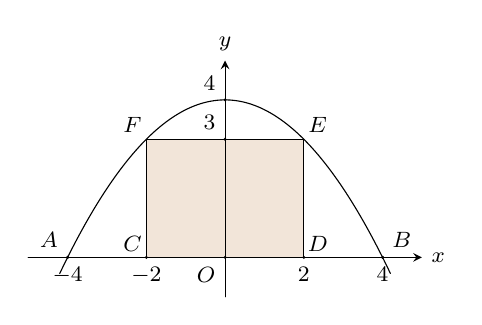
\begin{tikzpicture}[>=stealth,line join=round,line cap=round,font=\footnotesize,scale=0.5]
		\draw[fill=brown!20](-2,0)node[shift={(135:2.5mm)}]{$C$}--(-2,3)node[shift={(135:2.5mm)}]{$F$}--(2,3)node[shift={(45:2.5mm)}]{$E$}--(2,0)node[shift={(45:2.5mm)}]{$D$};
		\draw[->] (-5,0)--(5,0) node[right] {$x$};
		\draw[->] (0,-1)--(0,5) node[above] {$y$};
		\draw [smooth,domain=-4.2:4.2,samples=100]plot(\x,{-0.25*(\x)^2+4});
		\fill (0,0)node[below left]{\footnotesize{$O$}}circle(1.2pt) (2,0)node[below]{\footnotesize{$2$}}circle(1.2pt) (-2,0)node[below]{\footnotesize{$-2$}}circle(1.2pt) (0,3)node[above left]{\footnotesize{$3$}}circle(1.2pt) (0,4)node[above left]{\footnotesize{$4$}}circle(1.2pt) (4,0)node[below]{\footnotesize{$4$}}circle(1.2pt) (-4,0)node[below]{\footnotesize{$-4$}}circle(1.2pt);
		\fill (4,0)node[above right]{\footnotesize{$B$}}circle(1.2pt) (-4,0)node[above left]{\footnotesize{$A$}}circle(1.2pt);
\end{tikzpicture}}
\noindent
Vậy $(P)\colon y=-\dfrac{1}{4}x^2+4$.\\
Hai điểm $A$, $B$ là giao điểm của $(P)$ với $Ox$ nên hoành độ thỏa mãn
$$-\dfrac{1}{4}x^2+4=0\Leftrightarrow x^2=16\Leftrightarrow\hoac{&x=4\\&x=-4.}$$
Do vậy nên $A(-4;0)$ và $B(4;0)$, suy ra $AB=8$m.}
\end{bt}
\begin{bt}%[0D3V1-6]%[Dự án đề kiểm tra khối 10-11 GHK2 NH23-24- Đợt 2 - Phan Anh]%[Đề 5 - KNTT]
	Xác định giá trị của $m$ để hàm số $f(x)=x^3+\left(m^2-1\right)x^2+2x+m-1$ là hàm số lẻ.
	\loigiai{Tập xác định: $\mathscr{D}=\mathbb{R}$. Ta có
		\begin{itemize}
			\item $\forall x\in\mathscr{D}\Rightarrow(-x)\in\mathscr{D}$.
			\item $f(-x)=-x^3+\left(m^2-1\right)x^2-2x+m-1$, $\forall x\in\mathscr{D}$.
		\end{itemize}
	Hàm số đã cho là hàm số lẻ khi và chỉ khi $f(-x)=-f(x)$, $\forall x\in\mathscr{D}$.
	\begin{eqnarray*}
		&\Leftrightarrow&-x^3+\left(m^2-1\right)x^2-2x+m-1=-\left[x^3+\left(m^2-1\right)x^2+2x+m-1\right],\forall x\in\mathscr{D}\\
		&\Leftrightarrow&2\left(m^2-1\right)x^2+2(m-1)=0,\forall x\in\mathscr{D}\\
		&\Leftrightarrow&\heva{&m^2-1=0\\&m-1=0}\Leftrightarrow m=1.
\end{eqnarray*}}
\end{bt}
\begin{bt}%[0D7V3-1]%[Dự án đề kiểm tra khối 10-11 GHK2 NH23-24- Đợt 2 - Phan Anh]%[Đề 5 - KNTT]
	Xác định số giá trị nguyên của $m$ để phương trình $\sqrt{x^2-x+m}=\sqrt{x-3}$ có hai nghiệm phân biệt.
	\loigiai{Biến đổi phương trình ta được
	$$\sqrt{x^2-x+m}=\sqrt{x-3}\Leftrightarrow\heva{&x-3\ge0\\&x^2-x+m=x-3}\Leftrightarrow\heva{&x\ge3\\&x^2-3x+m+3=0.\quad(*)}$$
	Phương trình đã cho có hai nghiệm phân biệt $\Leftrightarrow(*)$ có hai nghiệm phân biệt thỏa $x\ge3$.
$$\Leftrightarrow\heva{&\Delta'=-m-2>0\\&x_1+x_2\ge6\\&\left(x_1-3\right)\left(x_2-3\right)\ge0}\Leftrightarrow\heva{&m<-2\\&2\ge6\text{ (vô lý)}\\&\left(x_1-3\right)\left(x_2-3\right)\ge0}$$
Vậy không có giá trị nguyên nào của $m$ thỏa mãn đề bài.}
\end{bt}
\begin{bt}%[0H9H2-3]%[Dự án đề kiểm tra khối 10-11 GHK2 NH23-24- Đợt 2 - Phan Anh]%[Đề 5 - KNTT]
	Cho ba điểm $A(-1;1)$, $B(2;1)$, $C(-1;-3)$. Tính chu vi và diện tích của tam giác $ABC$.
	\loigiai{Ta có $AB=\sqrt{3^2+0^2}=3$, $AC=\sqrt{0^2+(-4)^2}=4$, $BC=\sqrt{3^3+4^2}=5$.\\
	Nhận thấy $AB^2+AC^2=BC^2$ nên $\triangle ABC$ vuông tại $A$.\\
Chu vi tam giác $ABC$ là $P=AB+AC+BC=12$.\\
Diện tích tam giác $ABC$ là $S=\dfrac{1}{2}\cdot AB\cdot AC=6$.}
\end{bt}
\begin{bt}%[0H9V3-5]%[Dự án đề kiểm tra khối 10-11 GHK2 NH23-24- Đợt 2 - Phan Anh]%[Đề 5 - KNTT]
	Trong hệ trục tọa độ $Oxy$, viết phương trình đường thẳng $\Delta$ đi qua điểm $A(5;1)$ và cách điểm $B(2;-3)$ một khoảng bằng $5$.
	\loigiai{Gọi $\overrightarrow{n}=(a;b)\ne\overrightarrow{0}$ là véc-tơ pháp tuyến của đường thẳng $\Delta$, $\Delta$ qua $A(5;1)$ nên có phương trình
	$$a(x-5)+b(y-1)=0\Leftrightarrow ax+by-5a-b=0.$$
Ta có
\begin{eqnarray*}
	&&\mathrm{d}(B,\Delta)=\dfrac{|2a-3b-5a-b|}{\sqrt{a^2+b^2}}=5\\
	&\Leftrightarrow&|-3a-4b|=5\sqrt{a^2+b^2}\\
	&\Leftrightarrow&(3a+4b)^2=25\left(a^2+b^2\right)\\
	&\Leftrightarrow&16a^2-24ab+9b^2=0\\
	&\Leftrightarrow&(4a-3b)^2=0\Leftrightarrow4a=3b.
\end{eqnarray*}
Chọn $a=3\Rightarrow b=4$. Suy ra $\Delta\colon3x+4y-19=0$ là đường thẳng cần tìm.}
\end{bt}
\begin{bt}%[0H9V4-7]%[Dự án đề kiểm tra khối 10-11 GHK2 NH23-24- Đợt 2 - Phan Anh]%[Đề 5 - KNTT]
	Một bánh xe đạp hình tròn khi gắn trên hệ trục tọa độ $Oxy$ có phương trình $(C)\colon(x+1)^2+(y+2)^2=16$. Người ta thấy một hòn sỏi $M$ bị kẹt trên bánh xe và một điểm $A$ nằm trên đũa xe cùng với tâm của đường tròn tạo thành một tam giác cân tại $A$ có diện tích bằng $4$. Khi bánh xe qua tròn thì điểm $A$ sẽ di chuyển trên một đường tròn có phương trình gì?
	\loigiai{\immini{Đường tròn $(C)\colon(x+1)^2+(y+2)^2=16$ có tâm $I(-1;-2)$ và bán kính $R=4$.\\
			Điểm $M$ nằm trên đường tròn nên $IM=4$.\\
			Gọi $H$ là trung điểm của $IM$, ta có $IH=\dfrac{1}{2}IM=2$.\\
			Tam giác $AIM$ cân tại $A$ nên $AH\perp IM$.\\
			Diện tích tam giác $AIM$ bằng $4$ nên
			$$\dfrac{1}{2}\cdot AH\cdot IM=4\Leftrightarrow AH=\dfrac{2\cdot4}{IM}=\dfrac{2\cdot4}{4}=2.$$}
		{\begin{tikzpicture}[>=stealth,line join=round,line cap=round,font=\footnotesize,scale=0.5]
				\path (0,0) coordinate (I)
				(0,-4) coordinate (M)
				(2,-2) coordinate (A)
				($(I)!(A)!(M)$) coordinate (H)
				;
				\draw (H)--(A)--(I)--(M)--(A);
				\draw (I) circle (4);
				\foreach \p / \r in {I/135,A/0,M/-90,H/180}
				\fill (\p) circle (1.2pt) node[shift={(\r:2mm)}]{$\p$};
	\end{tikzpicture}}
\noindent
Tam giác $IHA$ vuông tại $H$ có $IA^2=IH^2+AH^2=2^2+2^2=8\Rightarrow IA=2\sqrt{2}$.\\
Vậy điểm $A$ nằm trên đường tròn tâm $I$, bán kính $IA=2\sqrt{2}$ nên có phương trình là $$(x+1)^2+(y+2)^2=8.$$}
\end{bt}
